%
% teil1.tex -- Beispiel-File für das Paper
%
% (c) 2020 Prof Dr Andreas Müller, Hochschule Rapperswil
%
% !TEX root = ../../buch.tex
% !TEX encoding = UTF-8
%
\section{Titel noch unklar
\label{helmholtz:section:teil1}}
\kopfrechts{Problemstellung}


\subsection{Planare Welle $\mathbf{Q} = 0$
\label{helmholtz:subsection:planarWelle}}

Planare Welle oder auch ebene Welle bedeutet, dass die Amplitude überall gleich gross ist und hat somit folgende Eigenschaften:

\begin{enumerate}
\item bei einer planaren Welle ist $P (\mathbf{r}) = P_0 = konst.\quad bzw. \quad \nabla P = 0$.
\item Aus der Gleichung \eqref{helmholtz:equationReaktiveIntensitaet} folgt $\mathbf{Q} = \mathbf{0}$.
\item sowie aus der Gleichung \eqref{helmholtz:equationAktiveIntensitaet} folgt $\mathbf{I} \neq \mathbf{0}$ da $ \nabla \phi$ parallel zur Ausbreitungsrichtung ist.
\item Schalldruck $P$ und Schall-Geschwindigkeit $v$ sind in Phase ($\phi = 0^{\circ}$).
\end{enumerate}

\begin{figure}
\centering
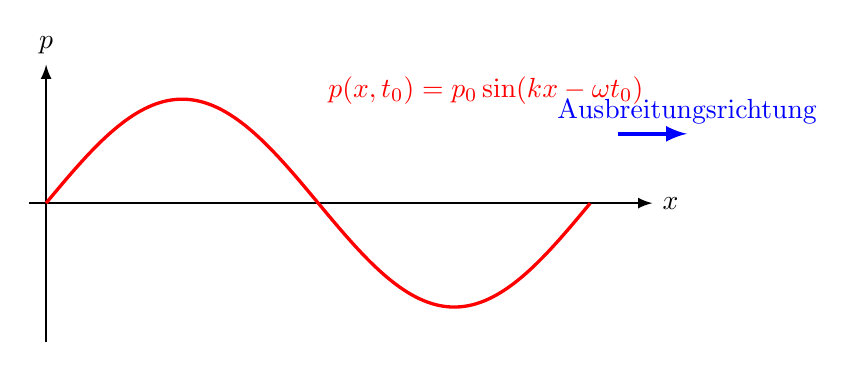
\begin{tikzpicture}[>=latex,thick,scale=1.1]

% Druckverlauf (rote Sinuskurve)
\draw[->] (-0.2,0) -- (7,0) node[right] {$x$};
\draw[->] (0,-1.6) -- (0,1.6) node[above] {$p$};

\draw[domain=0:6.283,samples=160,smooth,very thick,red]
  plot(\x,{1.2*sin(deg(\x))});

% Pfeil für Ausbreitungsrichtung
\draw[ultra thick,->,blue] (6.6,0.8) -- ++(0.8,0);
\node[blue,above] at (7.4,0.8) {Ausbreitungs\-richtung};

% Beschriftungen
\node[right,red] at (3.14,1.3) {$p(x,t_0)=p_0\sin(kx-\omega t_0)$};

\end{tikzpicture}
\caption{Ebene fortschreitende Welle: Druck und Geschwindigkeit $v$ sind überall in Phase ($\mathbf Q=0$).}
\end{figure}

\begin{equation}
	\mathbf{I}_c ~(\mathbf{r}) = \underbrace{\mathbf{I}~(\mathbf{r})}_{\textit{aktive Intensität}} + \underbrace{ \cancel{j\,\mathbf{Q}~(\mathbf{r})}}_{\textit{reaktive~Intensität}~=~0}.
	\label{helmholtz:equationIntensitaetComplexplanar}
\end{equation}	


\subsection{stehende Welle $\mathbf{I} = 0,\mathbf{Q} \neq 0$
\label{helmholtz:subsection:stehendeWelle}}

Bei einer stehenden Welle überlagern (Superposition) sich zwei gleiche planare Wellen mit gleicher Amplitude in entgegengesetzter Richtung und hat folgende Charakteristik:

\begin{enumerate}
\item an jedem Punkt ist entweder  $P = maximal$ und $v = 0$ bei einem Bauch (Darstellung) oder $P = 0$  und $ v = maximal$ bei einem Knoten (Darstellung).
\item fehlt noch was ??
\item Schalldruck $P$ und Schall-Geschwindigkeit $v$ sind 90\textdegree phasenverschoben ($\phi = 90^{\circ}$).
\end{enumerate}

\begin{figure}
\centering
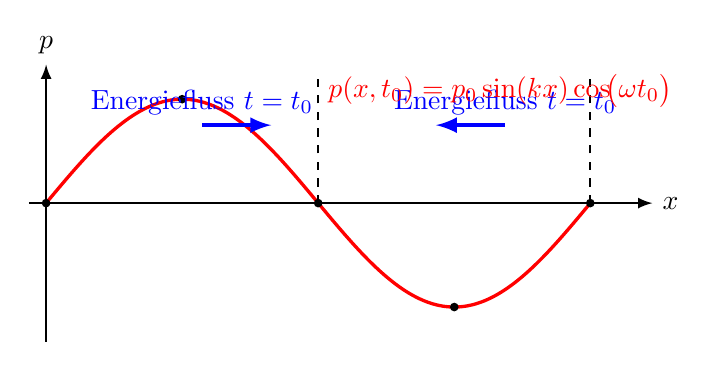
\begin{tikzpicture}[>=latex,thick,scale=1.1]

% Achsen
\draw[->] (-0.2,0) -- (7,0) node[right] {$x$};
\draw[->] (0,-1.6) -- (0,1.6) node[above] {$p$};

% Druckverlauf stehende Welle (rote Sinus)
\draw[domain=0:6.283,samples=160,smooth,very thick,red]
  plot(\x,{1.2*sin(deg(\x))});

% Knoten- und Bauchmarkierungen
\foreach \kk in {0,3.1415,6.283} {
  \draw[dashed] (\kk,0) -- (\kk,1.5);
  \fill[black] (\kk,0) circle(0.05);        % Druckknoten
}
\foreach \bb in {1.5708,4.7124} {
  \fill[black] (\bb,{1.2*sin(deg(\bb))}) circle(0.05);   % Druckbauch
}

% Hin‐ und Her-Energiepfeile
\draw[ultra thick,<-,blue] (4.5,0.9) -- ++(0.8,0);
\draw[ultra thick,->,blue] (1.8,0.9) -- ++(0.8,0);

\node[blue,above] at (1.8,0.9) {Energiefluss $t=t_0$};
\node[blue,above] at (5.3,0.9) {Energiefluss $t=t_0$};

% Beschriftung
\node[right,red] at (3.14,1.3) {$p(x,t_0)=p_0\sin(kx)\cos\!\bigl(\omega t_0\bigr)$};

\end{tikzpicture}
\caption{Stehende Welle: Druck und Geschwindigkeit sind an jedem Ort um $90^\circ$ phasenversetzt ($\mathbf I=0,\ \mathbf Q\neq0$).}
\end{figure}

\begin{equation}
	\mathbf{I}_c ~(\mathbf{r}) = \underbrace{\cancel{\mathbf{I}~(\mathbf{r})}}_{\textit{aktive Intensität}~=~0} + \underbrace{j\,\mathbf{Q}~(\mathbf{r})}_{\textit{reaktive~Intensität}}
	\label{helmholtz:equationIntensitaetComplexStehend}
\end{equation}	